% =====================================================================
%  Research proposal (standalone, single-file) — PRIMARY track
%  Inter-Animal Mask-Contact Geometry for Social Behaviour Recognition
%  Build:  ../build.sh proposal     (Tectonic + Ghostscript-normalise)
% =====================================================================
\documentclass[11pt]{article}

\usepackage[a4paper,margin=2.4cm]{geometry}
\usepackage{iftex}
\ifPDFTeX
  \usepackage[T1]{fontenc}
  \usepackage[utf8]{inputenc}
  \IfFileExists{lmodern.sty}{\usepackage{lmodern}\usepackage{microtype}}{}
\else
  \usepackage{fontspec}
  \IfFileExists{microtype.sty}{\usepackage{microtype}}{}
\fi
\usepackage{amsmath,amssymb}
\usepackage{booktabs}
\usepackage{enumitem}
\usepackage{caption}
\usepackage[dvipsnames]{xcolor}
\usepackage{tikz}
\usetikzlibrary{positioning,arrows.meta,fit,backgrounds,calc}
\usepackage[colorlinks=true,linkcolor=NavyBlue,citecolor=NavyBlue,urlcolor=NavyBlue]{hyperref}

\setlist{nosep,leftmargin=1.4em}
\captionsetup{font=small,labelfont=bf}

\title{\textbf{Inter-Animal Contact Geometry from Segmentation Masks}\\[2pt]
\large Do mask-derived contact features beat keypoint-hull geometry\\ for mouse
social-behaviour recognition?}
\author{Kostiantyn Boiar\\[2pt]
\small MSc thesis proposal, University of Glasgow}
\date{\today}

\begin{document}
\maketitle

\begin{abstract}
\noindent Automated recognition of \emph{social} animal behaviour — chasing, huddling,
investigating — hinges on the geometry of how two bodies meet. The field reads that geometry
from \emph{keypoint hulls}: convex polygons over a handful of pose keypoints, used by tools
such as SimBA~\cite{simba} and MARS~\cite{mars}. But a hull over sparse keypoints is crudest
\emph{exactly during contact}, when keypoints occlude, swap, or hallucinate and the polygon
smooths over the real boundary where two silhouettes touch. This proposal asks a sharp,
testable question: does \emph{inter-animal contact geometry derived from segmentation masks}
(mask IoU/overlap, contact-boundary length) add signal over keypoint-hull geometry for
social-behaviour recognition? We test it on the MABe22 mouse-triplet
benchmark~\cite{mabe22} with SAM\,2~\cite{sam2} as the enabling segmentation technology, every
heavy model frozen, and a single small head trained on cached features. Shape-from-silhouette
is \emph{not} claimed novel — it is established in human action and gait
recognition~\cite{bobickdavis,spacetimeshapes,gaitsurvey}; the contribution is, to our
knowledge, the first use of \textbf{mask-contact geometry} as an explicit behavioural feature,
in a clean head-to-head against the hull geometry the field already uses. The answer is
interpretable either direction.
\end{abstract}

% ---------------------------------------------------------------------
\section{Background and motivation}
% ---------------------------------------------------------------------
Recognising what animals are \emph{doing} from video underpins neuroscience and ecology, and
\emph{social} behaviours — where two or more animals interact — are both the most scientifically
interesting and the hardest to read. The defining signal of a social behaviour is
\textbf{geometric}: how close two bodies are, how much they overlap, where they touch.

The standard way to compute that geometry is from \textbf{pose keypoints}. Tools such as
SimBA~\cite{simba} build a convex \emph{hull} (polygon) over each animal's keypoints and derive
features like polygon percentage overlap and difference-area; MARS~\cite{mars} similarly derives
relational features from tracked keypoints for mouse social behaviour. This works, but it inherits
the weakness of sparse pose \emph{precisely when it matters most}. During close contact —
mounting, huddling, anogenital investigation — keypoints occlude one another, the tracker swaps
identities between near-identical animals, and a hull over a few noisy points bears little
relation to the true contacting surface. The crudeness of the representation peaks exactly at the
moment the behaviour is defined.

A \textbf{segmentation mask} does not have this failure mode: it captures the animal's full 2D
extent and, between two masks, the actual boundary where the silhouettes meet. Silhouette-based
shape is itself an old, well-validated idea — motion-energy/history templates with Hu
moments~\cite{bobickdavis}, ``actions as space-time shapes''~\cite{spacetimeshapes}, and the
entire field of gait recognition~\cite{gaitsurvey}. What changed is the \emph{extraction}: the
classical silhouette came from background subtraction against a static clean background, which
multi-animal lab/field video denies. \textbf{SAM\,2}~\cite{sam2} — promptable, video-propagated
instance segmentation — recovers a tracked foreground silhouette where the classical mechanism
fails. That makes mask-based contact geometry newly \emph{computable}, and nobody has yet used it
as a behavioural feature.

Two adjacent results sharpen the case. On the MammAlps wildlife benchmark, adding a static
\emph{scene/background} segmentation map did not merely fail to help — it \emph{degraded}
recognition (video-only class-average mAP fell from $0.453$ to $0.403$). PanAf-FGBG~\cite{panaf}
showed wildlife models over-rely on behaviour-correlated background and generalise poorly across
cameras, using SAM\,2 masks to \emph{erase} the animal and study the background. Both motivate
the \emph{opposite} move: keep the foreground geometry and discard the background.

% ---------------------------------------------------------------------
\section{Research questions and hypotheses}
% ---------------------------------------------------------------------
\begin{description}[leftmargin=2.4em,style=nextline]
  \item[RQ3 (primary)] Does \emph{mask-derived inter-animal contact geometry} (mask IoU/overlap,
    contact-boundary length) improve recognition of social/contact behaviours over the
    \emph{keypoint-hull geometry} the field uses?
  \item[RQ4 (insurance)] Is a shape/geometry representation more robust under \emph{background
    shift} (unseen cameras) than background-contaminated RGB features — the inversion of
    PanAf-FGBG? Publishable even if in-distribution accuracy is flat.
  \item[RQ1 (redundancy)] Does explicit mask geometry add anything \emph{over a frozen VideoMAE},
    which already ``sees'' the silhouette in pixels? (Confronted directly in the fusion stage.)
\end{description}

\noindent\textbf{Hypothesis.} Mask-contact geometry carries contact information that
keypoint-hull geometry captures only crudely, with the gap largest on the deepest-contact
behaviours. Fusing it will (i) beat the hull baseline head-to-head on contact behaviours, (ii)
show its clearest per-behaviour gains where keypoints occlude/swap, and (iii) degrade more
gracefully than RGB under background shift.

% ---------------------------------------------------------------------
\section{Proposed approach}
% ---------------------------------------------------------------------
\paragraph{Dataset.} \emph{MABe22 mouse-triplet}~\cite{mabe22}, the labelled \emph{submission}
split (the one that ships video, keypoints \emph{and} labels; verified by inspection):
\textbf{1{,}830 one-minute sequences} at 30\,Hz (1{,}800 frames each; 224$\times$224 grayscale
top-view), three near-identical mice, and \textbf{dense framewise binary labels} for four social
behaviours — \texttt{chases}, \texttt{huddles}, \texttt{oral\_oral\_contact} (oral contact),
\texttt{oral\_genital\_contact}. The behaviours are heavily imbalanced (huddle $\approx$8\,\%,
chase $\approx$0.05\,\% of frames positive), so we report \textbf{average precision} alongside F1
and class-balance at train time. Multi-animal contact is native here, which single-animal wildlife
clips (MammAlps) cannot provide; MammAlps is retained as a secondary single-animal /
background-robustness setting.

\paragraph{Keypoints — given, not estimated.} The dataset ships per-frame tracked pose as an array
$K \in \mathbb{R}^{T\times 3 \times 12 \times 2}$ (1{,}800 frames $\times$ 3 mice $\times$ 12
keypoints $\times$ $x,y$). We run \emph{no} pose estimation. Crucially, \textbf{both geometry
conditions start from these same keypoints}, so the comparison isolates the \emph{representation}
(sparse polygon vs.\ full silhouette), not the pose source.

\paragraph{Masks — SAM\,2 prompted by the keypoints.} For each mouse $i$ at frame $t$ we turn its
12 keypoints into SAM\,2 prompts — the keypoints as positive point prompts plus a tight box from
their extent — run SAM\,2 once, and \emph{propagate} the mask across the clip for temporal and
identity consistency, yielding one binary mask $M_i^t$ per mouse per frame. SAM\,2 is inference-only
(Table~\ref{tab:frozen}); masks (or the geometry derived from them) are cached once. Whether the
three masks stay \emph{separate and identity-stable through the contact frames} is the single
make-or-break risk, settled by the week-1 pilot (\S6).

\paragraph{The two geometry conditions (identical downstream).} From the same per-frame inputs we
compute, for each of the three mouse-pairs $(a,b)$, a small contact-feature vector — once from
\emph{hulls} (baseline) and once from \emph{masks} (novel):
\begin{itemize}
  \item \textbf{Hull contact geometry (baseline — SimBA/MARS).} Take each mouse's convex hull
    $H_i^t=\mathrm{conv}(K_i^t)$, a polygon over its 12 keypoints. Per pair: overlap ratio
    $O_{ab}=\lvert H_a\cap H_b\rvert / \lvert H_a\cup H_b\rvert$ (SimBA \texttt{polygon\_pct\_overlap}),
    difference-area, centroid distance, and minimum inter-keypoint distance. Polygon algebra via
    \texttt{shapely}; essentially free.
  \item \textbf{Mask contact geometry (novel).} From the two binary masks, the silhouette overlap
    $\mathrm{IoU}_{ab}=\lvert M_a\cap M_b\rvert / \lvert M_a\cup M_b\rvert$ and the
    \emph{contact-boundary length}
    $L_{ab}=\bigl\lvert\,\partial M_a \,\cap\, (M_b \oplus B_r)\,\bigr\rvert$ — the count of
    mouse-$a$ boundary pixels lying within $r$ px of mouse-$b$'s mask ($\partial$\,=\,boundary,
    $\oplus B_r$\,=\,dilation by radius $r$), i.e.\ \emph{how much of the two silhouettes physically
    touch}. Plus per-mouse \textbf{shape descriptors} for the posture side: area, aspect ratio,
    solidity (area\,/\,convex-hull area), and the seven Hu moments.
\end{itemize}
Each condition yields a per-frame vector (3 pairs $\times$ pair-features, $+$ 3 mice $\times$
shape-features) fed to a \textbf{tiny temporal encoder $+$ small head / linear probe}. Head
capacity is held \emph{identical}; the \emph{only} thing that changes between baseline and novel
condition is whether pair-overlap comes from a hull polygon or a mask — so any gain reflects
information, not parameters. The mechanistic bet: $O_{ab}$ (hull) is crudest \emph{exactly} during
deep contact, where keypoints occlude/swap and the polygon smooths over the true boundary, whereas
$\mathrm{IoU}_{ab}$ and $L_{ab}$ (mask) read the actual contacting surface.

\begin{table}[h]
\centering\small
\begin{tabular}{@{}lll@{}}
\toprule
Component & Pretrained model (frozen) & Role \\
\midrule
Masks    & SAM\,2~\cite{sam2}              & frame $+$ keypoint prompt $\rightarrow$ per-mouse \emph{mask} \\
Appearance & VideoMAE (Kinetics)           & clip $\rightarrow$ embedding (fusion / redundancy test) \\
Geometry & — (computed from masks/keypoints) & mask IoU, contact-boundary; hull overlap (baseline) \\
\bottomrule
\end{tabular}
\caption{Frozen building blocks. SAM\,2 is inference-only (never trained); the geometry features
are deterministic; only a small head / linear probe is trained. The \emph{keypoint-hull} geometry
(SimBA/MARS-style) is the comparison condition and is essentially free from the given keypoints.}
\label{tab:frozen}
\end{table}

\begin{center}
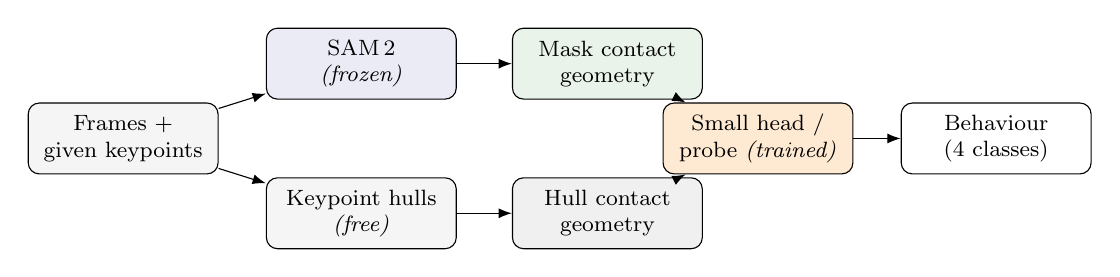
\begin{tikzpicture}[>=Latex,
  box/.style={draw, rounded corners, align=center, font=\footnotesize, inner sep=3pt,
              minimum height=0.9cm, text width=2.2cm}]
  \node[box, fill=black!4]   (in)   {Frames $+$\\given keypoints};
  \node[box, fill=NavyBlue!8, right=0.6cm of in, yshift=0.95cm]  (sam)  {SAM\,2\\\textit{(frozen)}};
  \node[box, fill=black!4, right=0.6cm of in, yshift=-0.95cm]    (hull) {Keypoint hulls\\\textit{(free)}};
  \node[box, fill=ForestGreen!10, right=0.7cm of sam]  (mgeo) {Mask contact\\geometry};
  \node[box, fill=black!6, right=0.7cm of hull]        (hgeo) {Hull contact\\geometry};
  \node[box, fill=BurntOrange!15, right=0.7cm of $(mgeo)!0.5!(hgeo)$] (head) {Small head /\\probe \textit{(trained)}};
  \node[box, right=0.6cm of head] (out) {Behaviour\\(4 classes)};
  \draw[->] (in) -- (sam); \draw[->] (in) -- (hull);
  \draw[->] (sam) -- (mgeo); \draw[->] (hull) -- (hgeo);
  \draw[->] (mgeo) -- (head); \draw[->] (hgeo) -- (head);
  \draw[->] (head) -- (out);
\end{tikzpicture}
\captionof{figure}{The head-to-head: identical-capacity head on \emph{mask} contact geometry
vs.\ \emph{hull} contact geometry (the field's baseline), from the same keypoints. Heavy models
frozen and cached; the mask branch is the novelty.}
\end{center}

\paragraph{Training \& protocol.} Only the head trains, on cached features (M4 / PyTorch MPS).
Class-balanced sampling; fixed seeds; report \textbf{mean $\pm$ 95\,\% CI over $\geq 5$ seeds}.
Modality dropout~\cite{actionmae} lets the geometry stream be dropped at test time; a heavier
DINOv2~\cite{dinov2} masked-crop embedding is held in reserve only if hand-crafted features
underperform.

% ---------------------------------------------------------------------
\section{Novelty (stated honestly)}
% ---------------------------------------------------------------------
The contribution is \emph{not} a new shape representation, and not ``fuse masks and tabulate it.''
It is, to our knowledge, the \textbf{first use of inter-animal segmentation-mask contact geometry
(mask IoU, contact-boundary length) as explicit features for social/contact behaviour
recognition}, in a controlled comparison against the keypoint-hull geometry the field already
uses. Each near neighbour is distinct:
\begin{itemize}
  \item \textbf{SimBA~\cite{simba} / MARS~\cite{mars}}: two-body geometry from \emph{keypoint
    hulls}, not masks. This is exactly our baseline condition; the experiment is mask-overlap vs
    hull-overlap, head to head.
  \item \textbf{Silhouette/shape methods}~\cite{bobickdavis,spacetimeshapes,gaitsurvey}: established
    in \emph{human} action and gait recognition, via background-subtraction silhouettes (single
    subject, clean background). We adapt the idea to \emph{multi-animal contact} using SAM\,2 where
    background subtraction is impossible — and gait is identity, not behaviour.
  \item \textbf{PanAf-FGBG~\cite{panaf}}: same tool (SAM\,2) for the \emph{opposite} purpose —
    masks used to \emph{erase} the animal and study the background. We keep the foreground geometry
    as a positive signal, and use their robustness finding as motivation.
\end{itemize}

% ---------------------------------------------------------------------
\section{Evaluation and pre-registered ablations}
% ---------------------------------------------------------------------
\paragraph{Eval contract (locked before modelling).} Framewise prediction of the four behaviours
(treated as independent binary tasks), over the annotated clips. \textbf{Leakage-safe split by
sequence} — every frame of a sequence stays in one split; never a random frame/window. Metric:
per-behaviour \textbf{F1} (the MABe convention) \emph{and} average precision (for comparability
with the MammAlps secondary track), macro-averaged over the four behaviours. The metric/split are
model-agnostic; the \emph{model} (a linear probe for the clean feature comparison, or the small
fusion head) is separate.

\paragraph{Pre-registered ablations.} To keep a small gain interpretable against seed noise, the
conditions and the success criterion are fixed \emph{in advance}: (a)~\textbf{hull geometry alone}
(the baseline); (b)~\textbf{mask geometry alone} vs (a) — the key isolation; (c)~\textbf{fusion}
(mask geometry on top of frozen VideoMAE) — the redundancy test (RQ1). Each runs $\geq 5$ seeds,
identical head capacity, reported as mean $\pm$ 95\,\% CI plus per-behaviour scores. \textbf{Success
is decided up front:} mask geometry helps iff it beats hull geometry with a 95\,\% CI excluding
zero \emph{and} a pre-registered minimum effect, or a clear per-behaviour win on the
deepest-contact behaviours (huddle, anogenital sniff). A scrambled-mask control rules out capacity
effects.

% ---------------------------------------------------------------------
\section{Risks and contingency}
% ---------------------------------------------------------------------
The novelty and the technical risk are the same thing: \textbf{can SAM\,2 keep three
near-identical mice as separate, identity-stable instances \emph{through the contact frames}}, when
masks tend to merge or swap? A \textbf{week-1 masking pilot} on the deepest-contact clips
(huddle, chase) settles it, with a written decision rule:
\begin{itemize}
  \item \textbf{PASS} (identities hold through contact) $\rightarrow$ proceed; contact geometry is
    the headline.
  \item \textbf{PARTIAL} (masks merge only in deepest contact) $\rightarrow$ treat a merge event as
    a coarse \emph{high-contact} feature alongside IoU/boundary on clean frames; proceed and say so.
  \item \textbf{FAIL} (frequent swaps/merges) $\rightarrow$ pivot the headline to
    \textbf{background-robustness (RQ4)} on the secondary MammAlps track, and report the
    contact-geometry attempt as an exploratory/negative result with the mask-quality analysis as
    evidence. The dissertation keeps a clean spine either way.
\end{itemize}
Compute is bounded: SAM\,2 is run once, behaviour-windowed and frame-subsampled ($\sim$5–6\,Hz),
caching derived geometry rather than raw masks; the trained head sees only cached vectors.

% ---------------------------------------------------------------------
\section*{Indicative timeline}
% ---------------------------------------------------------------------
\noindent
\begin{tabular}{@{}rl@{}}
\textbf{Wk 1} & Acquire MABe22; lock the label/eval contract; \textbf{masking pilot + decision}.\\
\textbf{Wk 2} & Scoped SAM\,2 mask cache (Kaggle); begin geometry features.\\
\textbf{Wk 3} & Finish contact-geometry + hull baseline extractor; head overfit sanity.\\
\textbf{Wk 4} & \textbf{Mask-geometry vs hull-geometry head-to-head} — first real result.\\
\textbf{Wk 5} & Per-behaviour analysis; multi-seed CIs; go/no-go on the MammAlps secondary track.\\
\textbf{Wk 6} & Fusion / VideoMAE-redundancy test; lock primary; begin secondary if reached.\\
\textbf{Wk 7} & Background-shift / robustness (RQ4); consolidate analysis.\\
\textbf{Wk 8} & Write-up; figures; package cached-feature pipeline + code.\\
\end{tabular}

% ---------------------------------------------------------------------
\begin{thebibliography}{99}
\bibitem{mabe22} J.~J.~Sun et al. \emph{The MABe22 Benchmark: Learning Multi-agent and Multi-species Behavior Representations.} ICML, 2023. arXiv:2207.10553.
\bibitem{simba} S.~R.~O.~Nilsson, N.~L.~Goodwin, J.~J.~Choong, et al. \emph{Simple Behavioral Analysis (SimBA): an open source toolkit for computer classification of complex social behaviors in experimental animals.} bioRxiv, 2020. doi:10.1101/2020.04.19.049452 (published in Nature Neuroscience, 2024).
\bibitem{mars} C.~Segalin, J.~Williams, T.~Karigo, et al. \emph{The Mouse Action Recognition System (MARS) software pipeline for automated analysis of social behaviors in mice.} eLife, 10:e63720, 2021. doi:10.7554/eLife.63720.
\bibitem{sam2} N.~Ravi et al. \emph{SAM\,2: Segment Anything in Images and Videos.} ICLR, 2025. arXiv:2408.00714.
\bibitem{panaf} O.~Brookes et al. \emph{The PanAf-FGBG Dataset: Understanding the Impact of Backgrounds in Wildlife Behaviour Recognition.} CVPR, 2025. arXiv:2502.21201.
\bibitem{bobickdavis} A.~F.~Bobick and J.~W.~Davis. \emph{The Recognition of Human Movement Using Temporal Templates.} IEEE TPAMI, 23(3):257--267, 2001. doi:10.1109/34.910878.
\bibitem{spacetimeshapes} L.~Gorelick, M.~Blank, E.~Shechtman, M.~Irani, and R.~Basri. \emph{Actions as Space-Time Shapes.} IEEE TPAMI, 29(12):2247--2253, 2007. doi:10.1109/TPAMI.2007.70711.
\bibitem{gaitsurvey} A.~Sepas-Moghaddam and A.~Etemad. \emph{Deep Gait Recognition: A Survey.} IEEE TPAMI, 45(1):264--284, 2023. doi:10.1109/TPAMI.2022.3151865.
\bibitem{actionmae} S.~Woo et al. \emph{Towards Good Practices for Missing Modality Robust Action Recognition (ActionMAE).} AAAI, 2023. arXiv:2211.13916.
\bibitem{dinov2} M.~Oquab et al. \emph{DINOv2: Learning Robust Visual Features without Supervision.} TMLR, 2024. arXiv:2304.07193.
\end{thebibliography}

\end{document}
